%-----------------------------------------------------------------------------------------
\clearpage
\section{Background Research}
%-----------------------------------------------------------------------------------------

In this section, a literature review is firstly introduced to present the most relevant works to this project. In the second part, previous systems in similar project is introduced. The third part provides an detailed analysis of the data characteristics.

\subsection{Literature Review}
This section introduced principles and techniques for data preprocessing and text data visualization.

Text Visualisation Browser \cite{Kucher2014} is an online tool providing the most comprehensive summary of published text visualization \cite{Cao2016a}. According to Text Visualisation Browser, from 1976 to 2017, there are 400 published text visualisation papers in total, in which 396 publications are aim to analyse text alignment. By searching "Word", there shows 20 publications, and "Translation" gets 16 results. Whereas when typing "Frequency" and "Weighting", each key word get 1 results. Also, key words such as "Machine learning, "Data Mining", "Natural Language Processing" got no publication collected. The results indicate that in text visualization domain, most researches focus on presenting alignment of texts. There are certain amounts of research focus on the topic such as "word analysis" and "translation", which is similar with this project. However, applying more specific techniques such as "Natural Language Processing" haven't been applied in text visualisation widely.

\subsection{Previous Systems}

In this section, interactive visualization of previsous system are introduced. For each research, data set and visualization techniques will be presented. Also, closely related work will be discussed in this section. 

\paragraph{Interactive Exploration of Versions across Multiple Documents}

\paragraph[]{}Work of \cite{Jong2008} provide a interactive visualization tool, MultiVersioner, to address the issues of comparing several versions of texts.


\subsection{Data Characteristics}

The data is major part of visualization. Along with the user experience, data plays an important role as "driving factor" with respect to the choice and attributes of the visualization method \cite{Laramee}. In this chapter, the data relevant to this project is analysed, including the type, size, format and characteristics of data. Also, a description of data preprocessing will be discussed. 

The data sets used in this project come from a collection of 57 different German translations of \emph{Othello}, which is contributed by Digital Humanities researchers working on a project in \cite{Tom2012}. To develop analytic tools and probe the translations in this corpus, the team has digitalized 32 translation versions, with the formats being normalized, texts being segmented, speech by speech and line by line. Also, the content of these 32 texts is a specific scene: the Act1, Scene 3 according to the English version of \emph{Othello} play as base text . Based on this corpus, we select 16 text files of German translation versions to study and focus on the words analysis. 

In this project, 17 text files are generated as corpus, among which 16 are German translation versions and 1 is the base text in English. All files are encoded as UTF-8 when converting from .docx file to .txt. file The number of words in each file are different according to the genres of text data (327 words at maximum, and 214 words at minimum). The data in each file has been preprocessed and organized line by line, and segmented speech by speech. 

Since the project is programmed in Java and focus on the words, the .txt is an appropriate format to store the data. Choosing .txt file as the data set is owing to following reasons:

\begin{itemize}
	\item \textbf{} The aim of this project focus on word processing, which require computer to read text literally, without applying complicated data processing techniques.
	\item \textbf{} Since the text data sets in the corpus are stored in .docx file which is difficult to read by Java directly, it is easy and safe to convert the texts into .txt file.
	\item \textbf{} There exits methods in Java API to read .txt data directly from files.
	\item \textbf{} Apart from the basic and simple information (year and author) of each version, there is no need to exact more information from the text. And because the data set in each version is not large, the computer can calculate the essential features of data, in a short time, every time the program is ran. 
\end{itemize}
\begin{figure}[h]
	\centering	
	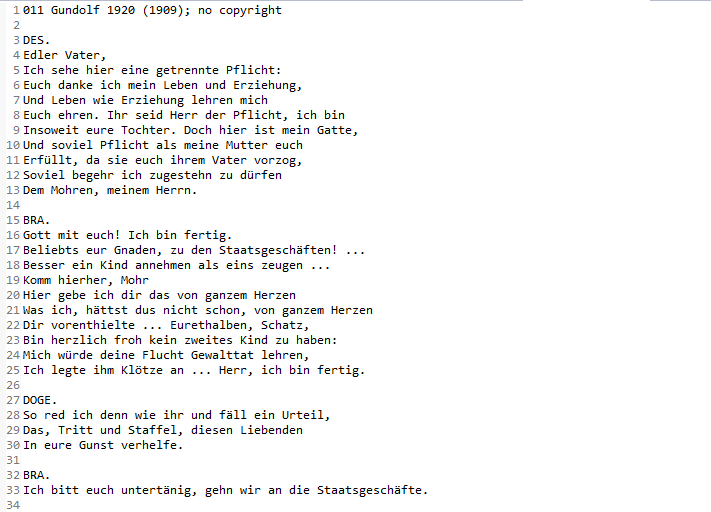
\includegraphics[width=13cm, height=9cm]{Figs/Data-example}\\[1ex]
	\caption{The text in .txt file. All data has been segmented and cleaned}
	\label{fig:dataExample}
\end{figure}




